\documentclass[11pt]{beamer}
\usetheme{Frankfurt}
\usepackage[utf8]{inputenc}
\usepackage[spanish]{babel}
\usepackage{amsmath}
\usepackage{amsfonts}
\usepackage{amssymb}
\usepackage{graphicx}
\usepackage{textcomp}
\usepackage{fancyvrb}

\setbeamercolor{headline}{bg=blue!30!white,fg=black}

\newcommand{\question}[1]
{
\begin{beamercolorbox}[sep=1mm, rounded=true, shadow=true]{headline}
#1
\end{beamercolorbox}
}

\author{Martin Ribelotta}
\title{Licencias de Software Libre}
\subtitle{Una introducción para principiantes}
\setbeamercovered{transparent} 
\setbeamertemplate{navigation symbols}{} 
\setbeamercovered{invisible}
%\logo{} 
%\institute{} 
%\date{}
%\subject{}
\begin{document}

\begin{frame}
\titlepage
\end{frame}

\begin{frame}
\frametitle{La forma de comerciar con Software}
\begin{block}{Conceptos basicos}
\begin{itemize}[<+-| alert@+>]
\item El software es un bien no material
\item No tiene las mismas restricciones que otros vienes fisicos
\item Su copia y distribución es cero o cercano a cero
\end{itemize}
\end{block}
\pause
\begin{exampleblock}{Concecuencias:}
\begin{itemize}[<+-| alert@+>]
\item El software no se vende
\item Se licencia para su uso
\item Similar a una obra literaria o musical
\item Protegida por derecho de autor
\item Para usar un software necesitamos permiso de su creador
\item Este permiso se conoce como ''licencia''
\end{itemize}
\end{exampleblock}
\end{frame}

\begin{frame}
\frametitle{Que es una licencia}
\begin{block}{Definición}
Una licencia es un contrato entre dos partes para el uso de un bien.
\end{block}

\begin{columns}

\column{.35\textwidth}
\begin{center}

\includegraphics[scale=0.3]{images/User1_icon.png}
\end{center}

\column{.20\textwidth}
\begin{center}

\includegraphics[scale=0.1]{images/document.png}
\end{center}

\column{.35\textwidth}
\begin{center}

\includegraphics[scale=0.3]{images/User1_icon.png}
\end{center}

\end{columns}
\end{frame}

\begin{frame}
\frametitle{Que es una licencia}
\begin{itemize}[<+-| alert@+>]
\item Ambas partes acuerdan terminos de uso
\item Puede tener una fecha limite o no
\item Puede restringirse el uso permitido
\item Puede restringirse los terminos de distrubicón
\item Cualquier cosa que este dentro de la ley
\end{itemize}
\end{frame}

\begin{frame}
\frametitle{Ejemplos de licencia}
\begin{block}{EULA de Microsoft Windows}
\begin{itemize}[<+-| alert@+>]
\item Copia privada limitada
\item Una instancia del producto por licencia (No VM)
\item Proibe explicitamente la copia a terceros
\item Restringe el tipo de hardware sobre el que corre (numero de procesadores y otros)
\item No ingenieria inversa
\item Licencia retroactiva (el contratante puede cambiar los terminos)
\item Muchas (muchas) mas que pueden no aplicar segun que circunstancia
\end{itemize}
\end{block}
\pause
\url{http://www.microsoft.com/argentina/public/kit_base/licenciamiento/licsemgt/mslicns/EULAs.htm}
\end{frame}

\begin{frame}
\frametitle{Licencias de Software Libre}
\begin{center}
\begin{Large}
Orientadas a resguardar las cuatro livertades basicas del software
\end{Large}
\end{center}
\pause

\begin{enumerate}[<+-| alert@+>]
\item[0] la libertad de \emph{usar} el programa, con cualquier propósito
\item[1] la libertad de \emph{estudiar} cómo funciona el programa y modificarlo
\item[2] la libertad de \emph{distribuir} copias del programa
\item[3] la libertad de \emph{mejorar} el programa y hacer públicas esas mejoras a los demás
\end{enumerate}
\onslide<6->{\textit {Richard Stallman, GNU BBS, 1986}}
\end{frame}

\begin{frame}
\frametitle{Licencias de Software Libre}
\begin{center}
\begin{Large}
Licencias con copyrigth {\Huge \copyright}
\end{Large}
\end{center}

\begin{itemize}[<+-| alert@+>]
\item Todas las licencias, tecnicamente, tienen copyright
\item Salvo las obras en dominio publico
\item Las demas, por ley, son propiedad de su creador
\item No es necesario el registro en ningun lado.
\item El derecho de autoria es inalienable
\item Junto con la autoria, se da el copyrigth por tiempo limitado
\item El licenciatario del software hace valer ese copyrigth al licenciar
\item Los entes registradores (de existir) son para dirimir (en caso de juicio) quien es el autor original
\end{itemize}

\end{frame}

\begin{frame}
\frametitle{Licencias de Software Libre}
\begin{center}
\begin{Large}
Licencias con copyleft {\Huge \textcopyleft}
\end{Large}
\end{center}

\begin{itemize}[<+-| alert@+>]
\item No es un termino legal
\item Es la forma de decirle a las licencias que \alert{aseguran} el cumplimiento de las cuatro livertades del software libre
\item Para esto establecen una serie de restricci\'ones sobre lo que se puede o no se puede hacer con el software
\item Igual que el EULA de Microsoft o cualquier otra empres
\item El exponente principal de estas licencias es la GPL y sus derivados
\end{itemize}
\end{frame}


\begin{frame}
\frametitle{Licencias de Software Libre}
\begin{center}
\begin{Large}
Licencias \alert{sin} copyleft {\Huge \textcopyleft}
\end{Large}
\end{center}

\begin{itemize}[<+-| alert@+>]
\item Permiten pero no garantizan las libertades del SL.
\item Se las llama licencias ''Permisivas'' debido a que, los terminos de licenciamiento, no poseen las restricciones de las licencias con copyleft
\item El exponente principal de estas licencias es la BSD aunque hay otras igual de importantes.
\end{itemize}
\end{frame}

\begin{frame}
\frametitle{Licencia GPL}
\begin{itemize}[<+-| alert@+>]
\item Creada por Richard Stallman en los 80 para el software de la fundaci\'on GNU
\item Licencia con Copyleft (a partir de aqu\'i se acu\~na este termino)
\item Pretende asegurar las cuatro livertades basicas planteadas por su creador
\end{itemize}
\end{frame}

\begin{frame}
\frametitle{Licencia GPL}
\begin{block}{¿Como lo hace?}
\begin{itemize}[<+-| alert@+>]
\item Permite \alert{expresamente} la distribuci\'on del software
\item Da el derecho de pedir una copia del codigo fuente \alert{a quien posea una copia} del software
\item Permite \alert{expresamente} la modificaci\'on, estudio y adaptaci\'on del codigo fuente
\item Permite el uso \alert{para cualquier proposito} del software \alert{sin restricci\'ones}
\item \alert{La unica} forma de distribuir copias o modificaciones del programa es \alert{bajo la misma licencia}
\item El trabajo \alert{Derivado} debe distribuirse con la misma licencia
\end{itemize}
\end{block}
\end{frame}

\begin{frame}
\frametitle{Licencia GPL}
\framesubtitle{Preguntas + frecuentes}

\question{¿Puedo vender software GPL?}
\pause
¡Totalmente! La Free Software Fundation anima a esta practica!
\pause
\question{Pero tengo que dar el codigo fuente!!!}
¡Totalmente!

Si es tuyo, lo pusiste como codigo GPL con esa intención

Sino, estas aprovechando codigo hecho por alguien con esa intención!!!

\end{frame}

\begin{frame}
\frametitle{Licencia GPL}
\framesubtitle{Preguntas + frecuentes}

\question{Pero alguien mas puede hacer negociós aparte de mi!!!}
\pause
Asi es!!! El software libre se basa en el altruismo y no en el secretismo!
\pause

\question{¿Tambien tengo que publicar mis modificaciones si lo solo lo uso yo?}
\pause
No estás obligado a hacerlo, la GPL solo cubre el hecho de distribuir la hobra

\end{frame}

\begin{frame}
\frametitle{Licencia (L)GPL}

\begin{block}{LGPL}

\begin{itemize}[<+-| alert@+>]
\item Extención de la GPL
\item Pensada para librerias de enlace dinamico
\item Permite \alert{combinar} software propietario con ''toolkits'' libres
\item Define ''interfaz de programación''
\item Todo lo que se haga a través de la ''interfaz de programación'' no esta cubierto por la (L)GPL
\item En todos los demas aspectos es igual a la GPL
\end{itemize}

\end{block}
\pause
\question{Si hago un programa que \alert{use} el API LGPL no tengo que cumplir la licencia al distribuir}
\pause
\question{Si \alert{modifico} el codigo LGPL es igual a modificar codigo GPL}

\end{frame}

\begin{frame}
\frametitle{Licencia BSD}
\begin{block}{BSD}
\begin{itemize}[<+-| alert@+>]
\item Escrita por la Universidad de Berkeley para su software
\item Berkeley Software Distributtion
\item Es la licencia mas simple sin copyleft que hay (en sus varias verciones)
\item Es facil de entender y a la vez es practica ante la ley
\item Pensada en preservar las libertades del programador antes que las del usuario
\end{itemize}
\end{block}
\end{frame}


\begin{frame}[fragile]
\frametitle{Licencia BSD}
Es tan corta que vale la pena leer su traducció

\begin{block}

Copyright (c) \emph{año}, \emph{titular del copyright}
Todos los derechos reservados.


La redistribución y el uso en las formas de código fuente y binario, con o sin
modificaciones, están permitidos siempre que se cumplan las siguientes condiciones:
\end{block}
\end{frame}

\begin{frame}
\frametitle{Licencia BSD}

\begin{enumerate}
\item Las redistribuciones del código fuente deben conservar el aviso de copyright
   anterior, esta lista de condiciones y el siguiente descargo de responsabilidad.
\pause
\item Las redistribuciones en formato binario deben reproducir el aviso de copyright
   anterior, esta lista de condiciones y la siguiente renuncia en la documentación
   y/u otros materiales suministrados con la distribución.
\pause
\item Ni el nombre de los titulares de derechos de autor ni los nombres de sus
   colaboradores pueden usarse para apoyar o promocionar productos derivados de
   este software sin permiso previo y por escrito.
\end{enumerate}
\end{frame}

\begin{frame}[fragile]
\frametitle{Licencia BSD}
\scriptsize
\begin{block}

ESTE SOFTWARE SE SUMINISTRA POR  \emph{TITULAR DEL COPYRIGHT} ''COMO ESTÁ'' Y CUALQUIER
GARANTÍA EXPRESA O IMPLÍCITAS, INCLUYENDO, PERO NO LIMITADO A, LAS GARANTÍAS
IMPLÍCITAS DE COMERCIALIZACIÓN Y APTITUD PARA UN PROPÓSITO DETERMINADO SON
RECHAZADAS. EN NINGÚN CASO \emph{TITULAR DEL COPYRIGHT} SERÁ RESPONSABLE POR NINGÚN
DAÑO DIRECTO, INDIRECTO, INCIDENTAL, ESPECIAL, EJEMPLAR O CONSECUENTE (INCLUYENDO,
PERO NO LIMITADO A, LA ADQUISICIÓN DE BIENES O SERVICIOS; LA PÉRDIDA DE USO, DE
DATOS O DE BENEFICIOS; O INTERRUPCIÓN DE LA ACTIVIDAD EMPRESARIAL) O POR
CUALQUIER TEORÍA DE RESPONSABILIDAD, YA SEA POR CONTRATO, RESPONSABILIDAD ESTRICTA
O AGRAVIO (INCLUYENDO NEGLIGENCIA O CUALQUIER OTRA CAUSA) QUE SURJA DE CUALQUIER
MANERA DEL USO DE ESTE SOFTWARE, INCLUSO SI SE HA ADVERTIDO DE LA POSIBILIDAD DE
TALES DAÑOS.
\end{block}

\end{frame}

\begin{frame}
\frametitle{Otras licencias BSD Like}

\begin{itemize}[<+->]
\item Licencia MIT: Usada por el Instituto Tecnológico de Massachusetts
\item Licencia Apache: Diseñada por la fundación Apache (ejemplo de uso Android)
\item Licencia CIAA: ''Traducción'' de la licencia BSD pensando en proyectos de Hardware
\end{itemize}
\end{frame}

\begin{frame}
\question{¿Cuando GPL o cuando BSD?}
\pause
\question{Redefiniendo: ¿Cuando Copyleft y cuando No copyleft?}
\pause
\question{Debate}
\end{frame}

\begin{frame}
\begin{figure}[hbtp]
\caption{Interacción entre licencias}
\centering
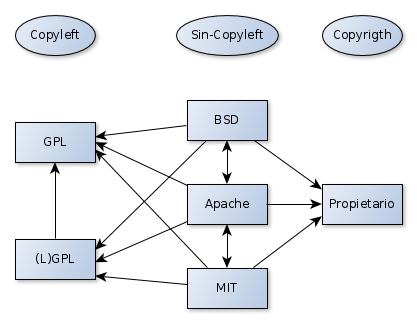
\includegraphics[scale=0.5]{images/lic-diagram.png}
\end{figure}

\end{frame}

\begin{frame}
\frametitle{Licencias de contenido}
\begin{block}{FDL: Free software documentation licence}
\begin{itemize}[<+->]
\item Licencia de documentación de la Free Software
\item Comparable en espiritu a GPL para documentos y articulos
\item Obra con copyleft (sus derivados deben segur la FDL)
\item Diseñada para manuales, libros de texto y material de referencia
\item Especifica secciones invariantes (Por ejemplo contribuidores)
\item Particularmente, esto ultimo hace impractica la licencia cuando muchos colaboran en el documento
\item Criticada por incluir reglas explicitas contra el DRM (pocon utiles e impracticas)
\end{itemize}
\end{block}
\end{frame}

\begin{frame}
\frametitle{Licencias de contenido: Creative Commons}
\begin{block}{CC}
\begin{itemize}[<+->]
\item La licencia CC \alert{NO EXISTE}
\item En su lugar existen varios sabores segun criterios señaladas por dos letras
\item BY: Reconocimiento al autor
\item SA: (Share Alike) o Compartir Igual (con la misma licencia)
\item NC: No comercial
\item ND: No permite hobras derivadas
\end{itemize}
\end{block}
\end{frame}

\begin{frame}
\frametitle{Licencias de contenido: Creative Commons}
\begin{block}{CC Ahora si!}
\begin{itemize}[<+->]
\item CC-BY: Equivale a una licencia BSD de contenido
\item CC-BY-SA: CC-BY con licencia virica (Share Alike)
\item CC-BY-NC: No comercial, "libre" pero no para vender
\item CC-BY-SA-NC: No comercial, con licencia virica (muy criticada)
\item CC-BY-ND: No derivadas, esto ya es contenido propietario del duro
\item CC-BY-NC-ND: No comercial, sin derivados. Contenido cerrado de toda la vida
\end{itemize}
\end{block}
\end{frame}

\begin{frame}
\frametitle{Licencias de contenido: Creative Commons}
\begin{block}{CC Ventajas y no tanto}
\begin{itemize}[<+->]
\item La licencia CC-BY tiene bastante sentido
\item La licencia CC-BY-SA es tambien muy util
\item Todas las -NC (non commercial) son criticadas pero todavia tienen sentido legal aunque menos practico
\item Las -ND (non derivative) son muy criticadas porque expresan lo mismo que el derecho de propiedad de autor
\item Corolario: No todo CC es libre
\item Corolario 2: No todo CC tiene sentido en todas las legislaciones de derecho de autor
\item CC-*-ND choca y se superpone con el derecho de autor en muchos paises.
\item Por supuesto, primero aplica el derecho de autor del pais en cuestion
\end{itemize}
\end{block}
\end{frame}

\begin{frame}
\question{¿Preguntas?}
\end{frame}

\begin{frame}
\question{¡¡¡Gracias!!!}
\end{frame}

\end{document}